\documentclass[8pt,conference,compsocconf]{IEEEtran}

\usepackage{geometry}
\geometry{margin=2cm,tmargin=2.2cm}
\usepackage{hyperref}
\usepackage{graphicx}	% For figure environment
\usepackage{xcolor}
\usepackage{amsmath}
\usepackage{amssymb}
\usepackage{booktabs}
\usepackage{dsfont}
\usepackage[caption=false]{subfig}
\usepackage{tabularx}
\usepackage{tikz}

\usepackage{multirow}


\begin{document}
\title{Project Report: Twitter Text Sentiment Prediction}

\author{
 Fereshte Mozafari, Mohammad Tohidi Vahdat, Ehsan Mohammadpour\\
 fereshte.mozafari@epfl.ch, mohammad.vahdat@epfl.ch, ehsan.mohammadpour@epfl.ch, \\
  \textit{EPFL, Switzerland}
}

\maketitle

\begin{abstract}
	Classification of Twitter message has been studied in the recent years in order to understand the sentiment of the messages as positive or negative ones.
	In this work, we use \textcolor{red}{type of neural net} neural networks to classify the sentiment of twitter messages. We use GloVe embedding to obtain feature matrix for the messages. In the proposed model, we construct a neural network by combining \textcolor{red}{CNN and RNN??} layers. The results show an improvement of $??$\% in the classification accuracy in comparison with regularized logistic regression. Finally, submitting our results in aicrowd.com shows \textcolor{red}{$84.4$}\% classification accuracy and \textcolor{red}{$0.85$} F1-score.
\end{abstract}
%\vspace{-0.3cm}
\section{Introduction}
Twitter sentiment classification has attracted increasing research interest in recent years \cite{8700266,8924403}.

define Twitter message as tweet
\par 
The rest of the paper is organized as follows. In Section \ref{sec:data}, we explain the data preprocessing in order to eliminate useless data. 

%In Section \ref{sec:model}, the model selection, the cross validation phase, and feature engineering are discussed. Section \ref{sec:results} shows the results of the selected model. Finally we conclude the paper in Section V.

\section{Data preprocessing}\label{sec:data}
An important step to have a decent classification is to export invaluable data from the given input. We are given two input files that include positive and negative tweets. To refine the input files, we did the preprocessing steps that are explained in the following subsections.
\subsection{Replacing emojis with appropriate words}
Emojis are commonly used in the messaging applications to express feeling or to shorten the tweet, e.g., one can replace "it was funny" by putting a "smiley" emoji. The idea is to replace the emojis with the corresponding main word, e.g., in the aforementioned example, the emoji is replaced with "funny".
\subsection{Removing numbers}
In the tweets, one may use some numbers; however, the numbers do not express the absolute sentiment of a tweet. One arbitrary value of a number can express positive or negative tweet. Consider the two sentences "I bought $1$ car" and "I have $1$ CHF", where both are using the number $1$. The former is expressing a positive feeling from a user informing they bought a car, while the later is considered as a negative one showing sadness of having little money. Here, we decided to remove the numbers, as they do not really expressing the sentiment of a tweet.
\subsection{Removing tags}
We have noticed the the files, two tags <user> and <url>, expressing the Twitter ID of a user and a URL\footnote{Uniform Resource Locator} of an external resource. They are not informative in the term of emotions; therefore, we removed them from the two input files.
\subsection{Removing stop-words}
A stop-word is a commonly used word such as "the", "a", "an", "in", to name but a few. These words not only do not help improving the classification, but also increase the feature space that is fed into the model. Therefore, we removed the stop-words which in turn caused an increase in the speed of model learning phase.

\section{Feature representation}\label{sec:embedding}
In the previous section, we capture the useful words in each tweet. The next main step to prepare the data for the training phase is to exploit the features of each word in a tweet. This technique is called "word embedding" in the context of Natural Language Processing research. Word embedding is a mathematical embedding from a space with many dimensions per word to a continuous vector space with a much lower dimension. 

To obtain such an embedding, firstly, we split each tweet into a vector of words. Then, we assign an id for each individual word, so that we convert each tweet into a vector of word ids. Secondly, we obtain an embedding of each word using pre-existing public word embedding solution, called GloVe \footnote{http://nlp.stanford.edu/projects/glove/}. There are three dimensions for GloVe that are $20$, $100$, and $300$. Although increasing the dimensionality of the embedding improves the accuracy of model, it also increases the time required to train a model. \textcolor{red}{In this project, we started with low-dimension embedding; however, for our final result, we use GloVe with $300$ dimensions to obtain a better result. The details comparison of the results are mentioned in Section \ref{sec:results}.}

\textcolor{red}{At the end of this step, we generated one vector of word ids for each tweet and a matrix for the vocabulary of the used words in the tweets where row $n$ of the matrix is an embedding for a word with id $n$.}

%\begin{enumerate}
%	\item tokenizing the tweets
%	\item assign numbers for each individual word, then for each tweet we have a sequence of numbers
%	\item for each word, we obtain an embedding this is already existed (like GloVe)
%	\item The obtained (tweet,numbering) pairs and (word, embedding vector) pairs are fed into one layer of neural network.
%\end{enumerate}
%\begin{itemize}
%	\item a
%\end{itemize}
%\section{Model training}\label{sec:model}
%In this section, we provide a description of the methods we have implemented to classify the tweets. We first describe Regularized Logistic Regression and Support Vector Machine  as the baseline methods; further, we focus more on the neural network methods since they are able to take into account the word sequence. The methods include Convolutional Neural Network (CNN) and Gated Recurrent Neural Network.
\section{Baseline} \label{sec:baseline}
%\begin{table}[t]
%	\centering
%	\caption{Comparison of accuracy over six different method of data training with maximum $500$ iterations.}
%	\begin{tabular}{|c|c|c|c|c|}
%		\hline
%		Model &Accuracy &$\gamma$ & $\lambda$\\
%		\hline
%		Gradient decent & $71.62$\%&$0.1$&-\\
%		\hline
%		Stochastic gradient decent &  $56.44$\% &$0.001$&-\\
%		\hline
%		Least square &  $71.72$\% &-&-\\
%		\hline
%		Ridge regression&  $71.72$\% &-&$1.0e{-5}$\\ 
%		\hline
%		Logistic regression &  $72.39$\% &$0.5$&-\\
%		\hline
%		Regularized logistic regression&  $72.39$\% &$0.5$&$1.0e{-5}$\\ 
%		\hline
%	\end{tabular}
%	\label{tab:6model_accuracy}
%\end{table}

We consider Regularized Logistic Regression (RLR) and Support Vector Machine (SVM) as two baseline methods. The main features of them are simplicity of implementation and fast training.

tfidf: tfidf is a document-term matrix in which each row represents a document (tweet in this project) and each column represent a term (word). For each row, only the terms in the corresponding document have a non-zero value; the value is a product of the term frequency and the inverse document frequency. The term frequency shows how frequent a term is in a document and the inverse document frequency indicates in how many documents the term is used.

\subsection{Regularized Logistic Regression}
This method is known to be used for classification purposes. We also rediscovered that in the first project of the course where RLR provide better accuracy in comparison with others including least square and regularized ridge regression. Therefore, we selected this method as one of the baseline methods. \textcolor{red}{The input should be described here. details of implementation is provided in Section \ref{sec:results}}


\subsection{Support Vector Machine}
SVMs methods are used for both regression and classification problems, specifically in the classification ones, they provide a maximum-margin decision boundary, which in turn causes the classification to be more robust. \textcolor{red}{The input should be described here. details of implementation is provided in Section \ref{sec:results}}



SVM is an 

\textcolor{red}{details of implementation is provided in Section \ref{sec:results}}
%\begin{table*}[ht]
%	\caption{Experimental results of using different deep learning and baseline methods.}
%	\def\arraystretch{1.1}\tabcolsep 5.2pt
%	\label{tab:results}
%		\begin{tabular}{|c|c||c|c|c||c|c|c|c||c||c|}
%			\hline
%			 \# of jets & Est. mass  &Test size	   &Original	& Polynomial& (F1)			&  (F1)+(F2)  & (F1)+(F3)+(F4)& (F1)+(F2)+(F3)+(F4)&\textbf{Final}&Imp.\\
%			\hline \hline
%			$0$ & \textit{NA}	  & $59263$ 	&$ 67.9$\%	& $95$\%	& $94.9$\%  & $95.1$\% & $95.2$\% & $95.3$\%  & $\textbf{95.3}$\% & $27.4$\%  \\
%			\hline
%			$0$ & $\checkmark$  	& $168195$   & $73.1$\%	 & $80.5$\% & $80.6$\%	& $81.2$\% & $81.5$\% & $81.$5\%  & $\textbf{81.5}$\% & $8.4$\%     \\
%			\hline
%			$1$ & \textit{NA}  	  & $17243$     & $69.8$\%  & $92$\%    & $92.5$\%  & $92.7$\% & $93$\%   & $93.1$\%   & $\textbf{93.2}$\% & $23.4$\%     \\
%			\hline
%			$1$ & $\checkmark$  			& $158095$   & $67.3$\%  & $78.5$\% & $79$\% 	 & $79.8$\% & $80$\%   & $80.4$\%   & $\textbf{80.4}$\% & $13.1$\%      \\
%			\hline
%			$2$ & \textit{NA} 	  & $6743$		& $82.9$\%  & $91.6$\% & $94.1$\% 	& $94.3$\% & $95.5$\% & $96$\%	   & $\textbf{97.7}$\% & $14.8$\% \\
%			\hline
%			$2$ & $\checkmark$  			& $107905$	& $72.8$\%  & $82.1$\% & $83.4$\% 	& $84$\%	& $84.2$\% & $84.5$\%	& $\textbf{84.5}$\%& $11.7$\%    \\
%			\hline
%			$3$ & \textit{NA} 	  & $3239$	    & $64.4$\% & $94.1$\% & $96.6$\%	& $97.5$\% & $98.6$\% & $99.1$\%  & $\textbf{99.9}$\% & $35.5$\%  \\
%			\hline
%			$3$ & $\checkmark$   			& $47555$	& $65.4$\%  & $81.9$\% & $81.8$\%	 & $84$\% 	 & $83.8$\% & $84.6$\%  & $\textbf{84.6}$\%  & $19.2$\%    \\
%			\hline
%			\hline
%			\multicolumn{2}{|c||}{Expected Accuracy}	  & - & $70.21$\%& $81.86$\% & $82.9$\%	 & $83.6$\%& $83.83$\% & $84.05$\%  & $\textbf{84.1}$\%  & $13.89$\%    \\
%			\hline
%	\end{tabular}
%\end{table*}
%In this section, first we describe how to select an appropriate model for the test data prediction. Then, we discuss about the cross validation among the training data and the extraction of hyper-parameters, i.e., the regularization parameter ($\lambda$) and the appropriate polynomial degree, to prevent under-fitting and over-fitting of the selected model .
%\vspace{-0.5cm}

\section{Deep Learning} \label{sec:deeplearning}
Deep learning allows computational models that are composed of multiple processing layers in order to learn representations of data with multiple levels of abstraction \cite{deeplearning}. We provide three deep learning architectures namely convolutional, gated recurrent neural network and long short-term memory. In the all aforementioned architectures, we have the following general layers:
\begin{itemize}
	\item The first layer of is an Embedding layer that we inject an embedding matrix produced from word embeddings to the model (Section \ref{sec:embedding})
	\item There are multiple layers corresponding to each deep learning architecture described later in this section.
	\item The one before the last layer is the drop-out layer. The goal of this layer is avoid over-fitting by dropping randomly a defined fraction of the hidden units in each iteration. In other words, since the number of learned parameters is increased in deep learning methods, it causes over-fitting of the model; drop-out layer is a solution to this issue. 
	\item The last layer is the dense layer which is a fully connected network; this layer generates the final prediction for the sentiment of the tweets. 
\end{itemize}


\subsection{Convolutional neural network}
Convolutional neural networks (CNN) use multiple layers with convolving filters that are applied to local features. In our CNN implementation, we have $5$ layers and we describe each one below:

%\begin{itemize}
%	\item The first layer of is an Embedding layer that we inject an embedding matrix produced from word embeddings to the model (Section \ref{sec:embedding})
%	\item The second layer is the convolutional layer with rectifier activation function. It extracts the local features around each word window with the size of $3$. 
%	\item The third layer is the max pooling layer. It extract the most important feature in the feature map obtained from the second layer.
%	\item The fourth is the drop-out layer. The goal of this layer is avoid over-fitting by dropping randomly a defined fraction of the hidden units in each iteration. In other words, since the number of learned parameters is increased in deep learning methods, it causes over-fitting of the model; drop-out layer is a solution to this issue. The fraction of dropping the hidden units is $0.25$ in this our CNN implementation.
%	\item The fifth layer is the dense layer which is a fully connected network; this layer generates the final prediction for the sentiment of the tweets. 
%\end{itemize}

\subsection{Recurrent neural network}
The idea behind RNNs is to make use of sequential information. In a traditional neural network we assume that all inputs (and outputs) are independent of each other. But for many tasks that’s a very bad idea. If you want to predict the next word in a sentence you better know which words came before it. RNNs are called recurrent because they perform the same task for every element of a sequence, with the output being depended on the previous computations and you already know that they have a “memory” which captures information about what has been calculated so far.
	\begin{figure}[t]
	\centering
	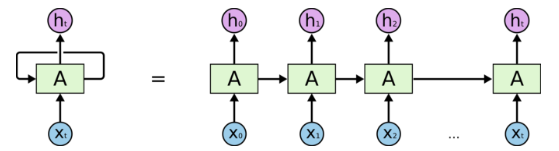
\includegraphics[width=0.9 \linewidth]{fig/rnn.png}
	\caption{An unrolled recurrent neural network. "A" is a recurrent unit (LSTM or GRU), $x_t$ is the input content and $h_t$ is the state output that is also used in the next computation round of the current state.}
	\label{fig:rnn}
\end{figure}
%\begin{itemize}
%	\item[(F1)] $CT$: cross term of two features $x_i$ and $x_j$, i.e., $x_i x_j$.
%	\item[(F2)] $\sqrt{CT}$: root square of the cross term.
%	\item[(F3)] $\arctan(CT)$: arctangent of the cross term.
%	\item[(F4)] $\sin(CT)$: sine of the cross term.
%	\item[(F5)] $CT^2$: square of the cross term
%\end{itemize}

\subsubsection{Gated recurrent neural network}

\subsubsection{Long Short-Term Memory}
LSTM’s have a Nature of Remembering information for a long periods of time is their Default behaviour.
\section{Results \& Discussion} \label{sec:results}
\begin{table}[t]
	\centering
	\caption{Experimental results of using different deep learning and baseline methods.}
	\begin{tabular}{|c|c|c|c|c|}
		\hline
		\multirow{2}{*}{Model} &\multicolumn{3}{|c|}{Accuracy of GloVe dimensions} \\
		\cline{2-4}
	 										& dim=$25$ &dim=$50$&dim=$300$\\
		\hline
		LSTM & $1$\%&$1$\%&$1$\%\\
		\hline
		CNN &  $1$\% &$1$\%&$1$\%\\
		\hline
		GRU &  $1$\% &$1$\%&$1$\%\\
		\hline
		SVM&  $1$\% &$1$\%&$1$\%\\ 
		\hline
		RLR&  $1$\% &$1$\%&$1$\%\\ 
		\hline
	\end{tabular}
	\label{tab:6model_accuracy}
\end{table}
%Table~\ref{tab:results} shows the incremental results of this project using regularized logistic regression with cross validation. The execution of cross validation for the $8$ sub-datasets results in finding $n=2$ and $\lambda=10^{-20}$ for each one. 
%%Using these two parameters leads to a significant improvement in the accuracy of the prediction which is illustrated in Table \ref{tab:results}.
%
%Due to space limitation, we did not put some intermediate results and tried to show the effect of manual feature augmentation described in Subsection \ref{sec:man_feature}. The last row shows the expected accuracy of the model over the test data set by calculation of weighted average based on the size of each data-subset.
%
%Our observation shows that adding each of the functions (F1) to (F4), beside the polynomial expansion, leads to an improvement in the predictions. However, addition of (F5)  just improves the prediction in two sub-datasets with number of jets equal to $2$ and $3$ and the estimated mass is \textit{NA}. The column \textit{Final} in Table~\ref{tab:results} shows the final results that utilize (F1) to (F4) for all sub-datasets and also (F5) for the aforementioned sub-datasets. The \textit{Imp.} column shows the amount of improvement in comparison with the original features (no polynomial and manual feature augmentation). We submitted the final predictions in the aicrowd.com with the team \textit{Panda\_feat\_Ah}, and obtained $83.7$\% accuracy and F1-score of $0.754$.
%
%We have to mention that the same procedure is done using 10-fold ridge regression. Although the local predictions show high accuracy, the result of the prediction over the test dataset was by far worse than the one with regularized logistic regression.


\section{Conclusion} \label{sec:conclusion}

For the implementation we used Keras library in python.
%In this project, we applied regularized logistic regression to a binary classification problem in order to predict whether a particle is a signal or a background noise, based on some measured features. We also showed that data preprocessing helps to improve the results of a machine learning model by removing meaningless data. We figured out the significant effect of polynomial feature expansion and the cross validation. It is noteworthy to mention that manual addition of some functions to the model substantially increased the model accuracy. To wrap up, the polynomial expansion as well as the feature augmentation led to an average improvement of $13.89$\% in the local final prediction.

\bibliographystyle{IEEEtran}
\bibliography{library}

\end{document}
